\documentclass[12pt, landscape]{article}
\usepackage[scaled=0.92]{helvet}
\usepackage{multicol}
\usepackage{calc}
\usepackage{ifthen}
\usepackage[landscape]{geometry}
%\usepackage{hyperref}

\usepackage{newtxtext} 

%for strikeout
\usepackage{ulem}

%For editing parbox
\usepackage[table]{xcolor}
%For editing itemise margins, reduce iterm separaion and list separation
\usepackage{enumitem}
% For math
\usepackage{amsmath,amsthm,amsfonts,amssymb}

%For pictures / figures
\usepackage{color,graphicx,overpic}
\graphicspath{ {./images/} }

%\usepackage{newtxtext} 
%\usepackage{amssymb}
%\usepackage[table]{xcolor}
%\usepackage{vwcol}
%\usepackage{tikz}
%\usepackage{wrapfig}
%\usepackage{makecell}

% Create cases
\usepackage{mathtools}

% Template: Cheatsheet with code enabled

%--------------------------- PACKAGES ABOVE --------------------------------------------------------------

\pdfinfo{
  /Title (ST2334.pdf)
  /Creator (Ger Teck)
  /Author (Ger Teck)
  /Subject ()
  /Keywords (tex)}

%% Margins for PAPER

% This sets page margins to .5 inch if using letter paper, and to 1cm
% if using A4 paper. (This probably isn't strictly necessary.)
% If using another size paper, use default 1cm margins.
\ifthenelse{\lengthtest { \paperwidth = 11in}}
	{ \geometry{top=.5in,left=.5in,right=.5in,bottom=.5in} }
	{\ifthenelse{ \lengthtest{ \paperwidth = 297mm}}
		{\geometry{top=1cm,left=1cm,right=1cm,bottom=1cm} }
		{\geometry{top=1cm,left=1cm,right=1cm,bottom=1cm} }
	}

% Turn off header and footer
\pagestyle{empty}

% for tight centres (less spacing)
\newenvironment{tightcenter}{%
  \setlength\topsep{0.5pt}
  \setlength\parskip{0.5pt}
  \begin{center}
}{%
  \end{center}
}

% Redefine section commands to use less space
\makeatletter
\renewcommand{\section}{\@startsection{section}{1}{0mm}%
                                {-1ex plus -.5ex minus -.2ex}%
                                {0.5ex plus .2ex}%x
                                {\normalfont\large\bfseries}}
\renewcommand{\subsection}{\@startsection{subsection}{2}{0.1mm}%
                                {-1explus -.5ex minus -.2ex}%
                                {0.5ex plus .2ex}%
                                {\normalfont\normalsize\bfseries}}
\renewcommand{\subsubsection}{\@startsection{subsubsection}{3}{0.1mm}%
                                {-1ex plus -.5ex minus -.2ex}%
                                {1ex plus .2ex}%
                                {\normalfont\small\bfseries}}
% change font
%\renewcommand{\familydefault}{\sfdefault}
%\renewcommand\rmdefault{\sfdefault}
\linespread{1.05}

\makeatother

% Define BibTeX command
\def\BibTeX{{\rm B\kern-.05em{\sc i\kern-.025em b}\kern-.08em
    T\kern-.1667em\lower.7ex\hbox{E}\kern-.125emX}}

% Don't print section numbers
\setcounter{secnumdepth}{0}

\setlength{\parindent}{0pt}
\setlength{\parskip}{0pt plus 0.5ex}

%% this changes all items (enumerate and itemize, reduce margins)
\setlength{\leftmargini}{0.5cm}
\setlength{\leftmarginii}{0.5cm}
\setlist[itemize,1]{leftmargin=2mm,labelindent=1mm,labelsep=1mm, itemsep = 1mm}
\setlist[itemize,2]{leftmargin=4mm,labelindent=1mm,labelsep=1mm, itemsep = 1mm}
\itemsep = 0mm
\setlist{nosep}

% Need Logo Picture
%Watermark Top Right
%\usepackage{atbegshi,picture}
%\AtBeginShipout{\AtBeginShipoutUpperLeft{%
 % \put(\dimexpr\paperwidth-1.2cm\relax, -1.2cm){\makebox[0pt][r]{\framebox{
\includegraphics[width = 0.3cm]{mountainbooks} Ger Teck}}}%
%}}


% -------------------------------------------------------------------------------

% START OF DOCUMENT HERE

\begin{document}
\raggedright
\footnotesize
\begin{multicols*}{3}



% multicol parameters
% These lengths are set only within the two main columns
%\setlength{\columnseprule}{0.25pt}
\setlength{\premulticols}{1pt}
\setlength{\postmulticols}{1pt}
\setlength{\multicolsep}{1pt}
\setlength{\columnsep}{2pt}

%% DOCUMENT NAME HERE
\begin{center}
     \Large{\textbf{ST2334 Summary Notes}} \\
\end{center}

AY23/24 Sem 1, github.com/gerteck

\section{1. Basic Probability Concepts }
\begin{itemize}
\item \textbf{Sample Space: $S$} All possible outcomes of stat. expt.
\item \textbf{Null Event}: Event that contains no element, empty set, $\varnothing$
\item \textbf{Axioms of Probability}:  \\ 
For any event X, $0 \leq P(X) \leq 1$.  $P(S) = 1$. \\
If $A \cap B = \emptyset$ (Mut Excl), $P(A \cup B) = P(A) + P(B)$. 
\item Finite sample space with equally likely outcomes: $P(A)$ = ($\frac{\# sample points A}{\#total sample points S}$). (e.g. birthday problem)
\end{itemize}

\subsubsection{Event Operation \& Relationships}
\begin{itemize}
\item \textbf{Event Operations:} Union, Intersection, Complement.
\item \textbf{Event Relationships:} Contained: {$A \subset B$} \\
Equivalence: {$A \subset B$ with $A \supset B \rightarrow A = B$} \\
Mutually Exclusive: {$A \cap B = \emptyset$}.
\item \textbf{De Morgan's Law:} {$(A \cup B)' = A' \cap B'$} and  {$(A \cap B)' = A' \cup B'$}
\end{itemize}

\subsubsection{Counting Methods}
\begin{itemize}
\item Multiplication Principle: (Sequential Events)
\item Addition Principle: (Pairwise Disjoin sets)
\item \textbf{Permutation}: {$_{n}P_{r} = \frac{n!}{(n-r)!}$}
\item \textbf{Combination}: {$\binom{n}{r} = \frac{n!}{(n-r)!r!}$}
\end{itemize}

\subsubsection{Conditional Probability}
• Understand conditional as reduced sample space. \\
\[P(B|A) = \frac{P(B \cap A)}{P(A)} = \frac{P(A|B)P(B)}{P(A)}\]

\subsubsection{Independence}
$A \perp B \leftrightarrow P(A \cap B) = P(A)P(B)$ \\
$A \perp B \leftrightarrow P(A|B) = P(A)$

% \vfill \null
\columnbreak


\subsubsection{Law of Total Probability}
\begin{itemize}
\item \textbf{Partition: }{If $A_1, \cdots, A_n$ mutually exclusive, $\bigcup _{i=1} ^{n} A_i = S$, then $A_1, \cdots, A_n$ are partitions.}
 \item If $A_1, \cdots, A_n$ are partitions of S, then for any event B:
    \[P(B) = \sum _{i=1} ^{n} P(B \cap A_i) = \sum _{i=1} ^{n} P(B|A_i)P(A_i)\]
\end{itemize}

\subsubsection{Bayes' Theorem}
Let $A_1, \cdots, A_n$ be partitions of S. For any event B:
\[P(A_k|B) = \frac{P(B|A_k)P(A_k)}{\sum _{i=1} ^{n} P(B|A_k)P(A_i)}\] 
For when $n = 2$, $\{A, A' \}$ becomes a partition of $S$.
\[P(A|B) = \frac{P(A)P(B|A))}{P(A)P(B|A) + P(A')P(B|A')}\] 

\section{2. Random Variables}
A function X, which assigns a real number to every s $\in$ S is
called a random variable. \\
• \textbf{Range space}: $Rx = \{x|x = X(s), s \in S\}$ \\
• Likewise, the set X $\in$ A, for A being a subset of R, is also a subset of $S: {s \in S : X(s) \in A}$.


\subsubsection{Probability Distribution}
Two main types of RV used in practice: discrete and continuous.
\begin{itemize}
    \item Probability assigned to each possible $X$
    \item Given RV $X$ with range of $R_x$:
        \subitem \textbf{Discrete: }{Numbers in $R_x$ are finite or countable}
        \subitem \textbf{Continuous: }{$R_x$ is interval}
\end{itemize}

\subsubsection{(Discrete) Probability Mass Function $f(x)$:}
\[
f(x)
    \begin{cases*}
        P(X=x), & for $x\in R_X$ \\
        0, & for $x\notin R_X$\\
    \end{cases*}
\]
\begin{enumerate}
	\item $f(x_i) = P(X = x_i) \geq 0$ for $x_i \in R_x$
      \item $f(x_i) = 0$ for $x_i \notin R_x$
      \item $\sum _{i=1} ^{\infty} f(x_i) = 1$ (PSum = 1)
      \item $\forall B \subseteq \mathbb{R}, P(X \in B) = \sum _{x_i \in B \cap R_x} f(x_i)$
\end{enumerate}

\subsubsection{(Continuous) Probability Density Function $f(x)$:}
\begin{itemize}
    \item {Given $R_x$ is interval. Quantifies probability that $X$ is in some range.}
    \item $p.f.$ must satisfy:
        \begin{enumerate}
            \item $f(x) \geq 0$, $f(x) = 0$ for $x \notin R_x$
            \item No need $f(x) \leq 1$ (Concerned with area)
            \item $\int _{R_x} f(x) dx = 1$ (Integration over $R_X$ = 1)
            \item $\forall a,b \text{ s.t. } a \leq b, P(a \leq X \leq b) = \int _{a} ^{b} f(x) dx$
        \end{enumerate}
    \item \textbf{Note:} $P(X = x_0) = \int _{x_0} ^{x_0} f(x) dx = 0$
    \item Hence, to check if a function is a pdf, \\
    	 1. $f(x) \geq 0$  for $x \in R_x$,  $f(x) = 0$ for $x \notin R_x$ \\
    	 2. $\int _{R_x} f(x) dx = 1$.
\end{itemize}

\subsection{Cumulative Distribution Function}
Describes distribution of a RV $X$: cumulative distribution function (cdf), applicable for discrete or continuous RV.
\[F(x) = P(X \leq x)\]
 $F(x)$ is non-decreasing and $0 \leq F(x) \leq 1$ \\
• Probability fn \& cumulative distribution fn have one-to-one correspondence. For any probability fn given, the cdf is uniquely determined, vice versa.

\subsubsection{CDF Discrete RV: Step Function $F(x)$}

    \[F(x) = \sum _{t \in R_x; t \leq x} f(t)\]
	\centerline{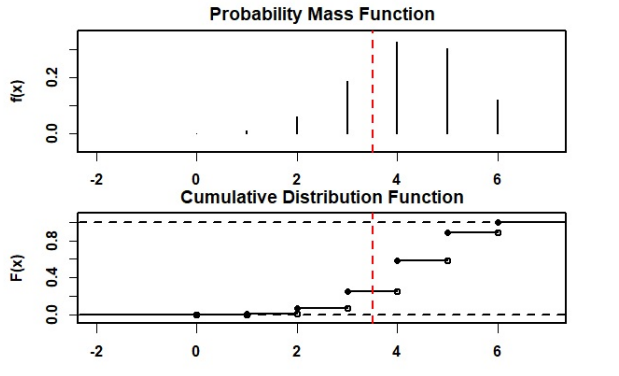
\includegraphics[width=0.5\linewidth]{cdfstep}}
    \begin{itemize}
       \item $P(a \leq X \leq b)=P(X \leq b)-P(X < a)$
       \item $P(a \leq X \leq b)=F(b)-F(a-)$
	\item $P(a \leq X \leq b) =  F(b) - \lim _{x \to a^-} F(x)$
       \item $0 \leq f(x) \leq 1$
       \item  c.d.f has to be \textbf{right continuous} (• ---)
    \end{itemize}

%\vfill \null
\columnbreak

\subsubsection{CDF Continuous RV: $F(x)$}
    \[F(x) = \int _{-\infty} ^{x} f(t) dt\]
    \[impt: f(x) = \frac{d(F(x))}{dx}\]
    \centerline{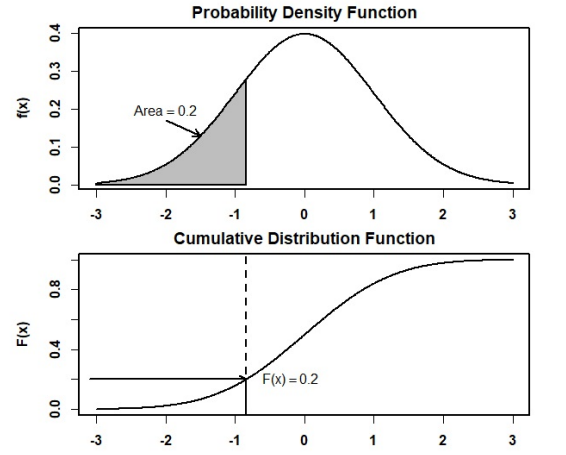
\includegraphics[width=0.5\linewidth]{cdfcontinuous}}
    \begin{itemize}
        \item $P(a \leq X \leq b) = P(a < X < b) = F(b) - F(a)$
        \item $0 \leq f(x)$. \\
         e.g. $f(x) = 3x^2$ is a valid $p.f.$ since $\int _{R_x} f(x) dx = 1$
    \end{itemize}
    
   
\subsection{Expectation $\mu$ \& Variance $\sigma$}
\subsubsection{Expectation of Random Variable: $\mu$ }
\begin{itemize}
    \item \textbf{Mean of discrete RV}: 
    \[\mu = E(X) = \sum _{x \in R_x} x_i f(x_i)\]
    \item \textbf{E.g.}: X discrete RV with p.m.f. $f(x)$ and range $R_X$ \\ 
     $\mu =$ $E(g(x)) = \sum _{x \in R_x} g(x)f(x)$
    
    \medskip
    \item \textbf{Mean of continuous RV}: 
    \[\mu = E(X) = \int _{x \in R_x} x f(x) dx\]
    \item \textbf{E.g.}: X continuous RV with p.d.f. $f(x)$ and range $R_X$ \\
    $\mu =$ $E(g(x)) = \int _{x \in R_x} g(x)f(x)dx$
    
    \smallskip
    \item \textbf{Properties of Expectation:}
    \item $E(aX + b) = aE(X) + b$
    \item Linearity of expectation: $E(X + Y) = E(X) + E(Y)$
\end{itemize}

\columnbreak

\subsubsection{Variance of Random Variable: $\sigma$}

\[\sigma_X^2 = V(X) = E[(X - \mu_X)^2]\]

\begin{itemize}
    \smallskip
    \item \textbf{Variance of discrete RV}: 
    \[V(X) = \sum _{x \in R_x} (x - \mu_X)^2 f(x)\]
    
    \medskip
    \item \textbf{Variance of continuous RV}: 
    \[V(X) = \int _{x \in R_x} (x - \mu_X)^2 f(x) dx\]
    
    \medskip
    \item $V(X) \geq 0$ and $V(X) = 0$ when $X$ is a constant
    \item $V(aX+b) = a^2V(X)$
    \item \textbf{alt. form:} $V(X) = E(X^2) - (E(X))^2$
    \item \textbf{Standard Deviation: }{$\sigma_X = \sqrt{V(X)}$}
\end{itemize}

% 3. JOINT DISTRIBUTIONS =================== 


\section{3. Joint Distributions}
\begin{itemize}
    \item Consider more than 1 RV simultaneously, 
    \item Given sample space $S$. Let $X$ and $Y$ be functions mapping $s \in S \to \mathbb{R}$: $(X, Y)$ is 2D random vector.
    \[\text{\textbf{Range spc:}} R_{X, Y} = \{(x,y) | x = X(s), y=Y(s), s \in S\}\]
    \item \textbf{Discrete 2D RV:} \\
    {\# of possible values of $(X(s), Y(s))$ finite / countable}
    \item \textbf{Continuous 2D RV}:  \\
    	{\# of possible values of $(X(s), Y(s))$ assume any value in some region of the Euclidean space $\mathbb{R}^2$}
    \item If both $X$ and $Y$ are discrete/continuous, then $(X, Y)$ is discrete/continuous respectively.
\end{itemize}

\subsection{Joint Probability Function}

\begin{itemize}
     \item \textbf{Joint Probability (mass) function, 2D discrete RV}:
    \[f_{X,Y} (x,y) = P(X = x, Y = y)\]
    \begin{itemize}
        \item $f_{X,Y} (x,y) \geq 0$ for any $(x,y) \in R_{X,Y}$
        \item $f_{X,Y} (x,y) = 0$ for any $(x,y) \notin R_{X,Y}$
        \item $\sum _{i=1} ^{\infty} \sum _{j=1} ^{\infty} P(X = x_i, Y = y_i) = 1$
        \item Let $A \subseteq R_{X, Y}$. $P((X,Y) \in A) = \sum \sum _{(x,y) \in A} f_{X, Y}(x,y)$
    \end{itemize}
     \item \textbf{Joint Probability (density) function, 2D cont. RV}:
    \[P(a \leq X \leq b, c \leq Y \leq d) = \int _a ^b \int _c ^d f_{X, Y} (x, y)dydx\]
    \begin{itemize}
        \item $f_{X,Y} (x,y) \geq 0$ for any $(x,y) \in R_{X,Y}$
        \item $f_{X,Y} (x,y) = 0$ for any $(x,y) \notin R_{X,Y}$
        \item $\int _{-\infty} ^{\infty} \int _{-\infty} ^{\infty} f_{X,Y} (x,y)dxdy = 1$ \\
        or equivalently:
        \item $\int _{} ^{} \int _{(x,y) \in R_{X,Y}} ^{} f_{X,Y} (x,y)dxdy = 1$
    \end{itemize}
\end{itemize}

\subsection{Marginal Probability Function}
Marginal distribution of $X$ is individual distribution of $X$, ignoring the value of $Y$. “Projection” of 2D function
$f_{X,Y}(x, y)$ to 1D function. \\
\medskip
Let $(X,Y)$ be 2D RV with joint probability function $f_{X,Y} (x,y)$:
\[\text{If $Y$ is \textbf{discrete}, } f_X(x) = \sum _y f_{X,Y} (x,y)\]
\[\text{If $Y$ is \textbf{continuous}, } f_X(x) = \int _{-\infty} ^\infty f_{X,Y} (x,y)dy\]

\begin{itemize}
    \item $f_Y (y)$ defined similarly
    \item $f_X(x)$ is a $p.f.$, satisfies all properties of prob. fn.
\end{itemize}

\subsection{Conditional Distribution}

Let $(X,Y)$ be 2D RV with joint probability function $f_{X,Y} (x,y)$. 
Then $\forall x$ s.t. $f_X(x) > 0$: ($X$ marg prob fn.) \\
\textbf{Conditional probability function of $Y$ given $X$ = $x$:}

\[f_{Y|X} (y|x) = \frac{f_{X,Y}(x,y)}{f_X (x)}\]

\begin{itemize}
    \item Intuition: Distribution of $Y$ given $X = x$
    \item Only defined for $x$ s.t. $f_X(x) > 0$
    \item $f_{Y|X} (y|x)$ is a $p.f.$ if we fix $x$, satisfies prop. of prob.fn.
    
    \medskip
    \item But, $f_{Y|X} (y|x)$ is not a $p.f.$ for $x$: No need for sum / integral over x = 1. Hence, \\
    	If $f_X (x) > 0$: $f_{X,Y} (x,y) = f_X (x)f_{Y|X} (y|x)$ \\
    	If $f_Y (y) > 0$: $f_{X,Y} (x,y) = f_Y (y)f_{X|Y} (x|y)$
    \item \textbf{Probability Y $\leq y$, Average $Y$ given $X = x$}
    \item $P(Y \leq y | X = x) = \int _{-\infty} ^y f_{Y|X} (y|x)dy$
    \item $E(Y|X=x) = \int _{-\infty} ^{\infty} y f_{Y|X} (y|x)dy$
\end{itemize} 
  
\columnbreak

% INDEPENDENT RANDOM VARIABLES ===========================
\subsection{Independent Random Variables}

\[X \perp Y: \forall x,y, f_{X,Y} (x,y) = f_X (x) f_Y (y)\]

\begin{itemize}
    \item Necessary condition: $R_{X,Y}$ must be a product space. \\ 
    i.e. $R_{X,Y} = \{(x, y)|x \in R_X ; y \in R_y\} = R_X  \times R_Y$ \\
    Else, dependent.
\end{itemize}

\subsubsection{Properties of Independent RV}
\textbf{For $X,Y$ independent RV:}
\begin{itemize}
    \item If $A,B \subseteq \mathbb{R}$, then events $X \in A$ and $Y \in B$ are independent:
    \[P(X \in A; Y \in B) = P(X \in A) P(Y \in B)\]
    \[P(X \leq x; Y \leq y) = P(X \leq x) P(Y \leq y)\]
    \item Then, $g_1(X)$ and $g_2(Y)$ are \textbf{independent}, for arbitrary $g$.
    \item \textbf{Conditional distribution} given Independence:
    \[f_X(x) > 0 \to f_{Y|X} (y|x) = f_Y(y)\]
    \[f_Y(y) > 0 \to f_{X|Y} (x|y) = f_X(x)\]
\end{itemize}

\subsubsection{To check independence}
\begin{enumerate}
    \item $R_{X,Y}$ is a product space. i.e. $R_X$ does not depend on $Y$, vice versa. (e.g. $ 0 < y < x $ is NOT a product space) 
    \item Additionally, \textbf{ $f_{X,Y} (x,y)$ = some $C * g_1(x)g_2(y)$ where $g_1$ depends on $x$ only and $g_2$ depends on $y$ only. }
\end{enumerate}    

\subsubsection{Marginal Distribution under Independence} 
\begin{itemize}
	\item Since, $f_{X,Y} (x,y) = f_X (x) f_Y (y)$ for independent RV, we derive marginal distribution by standardising $g_1(x)$ and $g_2(y)$.
	\item For discrete: $f_X (x) = \frac{g_1(x)}{\sum _{t \in R_X} g_1 (t)}$
    	\item For continuous: $f_X (x) = \frac{g_1(x)}{\int _{t \in R_X} g_1 (t)dt}$
\end{itemize}

\columnbreak

% EXPECTATION & COVARIANCE ==============

\subsection{Expectation of a Random Vector}

Given \textbf{2 variable function $g(x,y)$:}
\begin{itemize}
\item If $(X,Y)$ is discrete:
\[E(g(X,Y)) = \sum _x \sum _y g(x,y) f_{X,Y} (x,y)\]
\item If $(X,Y)$ is continuous:
\[ E(g(X,Y)) = \int _{-\infty} ^\infty \int _{-\infty} ^\infty g(x,y) f_{X,Y} (x,y) dydx\]
\item If $X \perp Y$: 
\[ E(XY) = E(X)E(Y) \]
\item (If $X \perp Y$, follows that $cov(X,Y) = 0$). However, converse not always true.
\end{itemize}

\subsection{Covariance}
\begin{itemize}
\item For random variables $X, Y$:
\[cov(X,Y) = E((X - E(X))(Y - E(Y)))\]
\item If $(X,Y)$ both \textbf{discrete}:
\[ cov(X,Y) = \sum _x \sum _y (x - \mu_X)(y - \mu_Y) f_{X,Y} (x,y)\]
\item If $(X,Y)$ both \textbf{continuous}: 
\[cov(X,Y) = \int _{-\infty} ^\infty \int _{-\infty} ^\infty (x - \mu_X)(y - \mu_Y) f_{X,Y} (x,y)dxdy\]

    \item \textbf{Alt:} $cov(X,Y) = E(XY) - E(X)E(Y)$
    \item \textbf{Hence, for}$X \perp Y \to cov(X,Y) = 0$. \\ (However, converse not always true).
    \item \textbf{Properties of covariance:}
    \item $cov(aX+b, cY+d) = (ac) cov(X,Y)$
    \item $V(aX+bY) = a^2V(X) + b^2V(Y) + 2ab*cov(X,Y)$
    \item $X \perp Y \to V(X \pm Y) = V(X) + V(Y)$ 
\end{itemize}

\columnbreak
 \vfill \null
 \columnbreak

% CHAPTER 4: Probability Distributions ==================================
% DISCRETE ==============
\section{4.1 Special Probability Distributions}
\begin{itemize}
\item \textbf{Discrete Distributions}: Study whole classes of discrete RVs that arise frequently in applications.
\end{itemize}

\subsection{Discrete Uniform Distribution}
\begin{itemize}
    \item If $X$ has values $x_1, x_2, \cdots, x_k$ with \textbf{equal probability}
    
    \[
f(x)
    \begin{cases*}
        \frac{1}{k}, & for $x = x_1, x_2, ..., x_k$ \\
        0, & otherwise\\
    \end{cases*}
\]
 
    \item \textbf{Expectation}: $\mu_X = E(X) = \sum_{i = 1} ^{k} x_i f_X (x_i) = \frac{1}{k} \sum x_i$
    \item \textbf{Variance}: $\sigma_X^2 = V(X) = E(X^2) - (E(X))^2 = \frac{1}{k} \sum x_i^2 - \mu_X^2$
\end{itemize}

\subsection{Bernoulli, $Ber(p)$}

\begin{itemize}
    \item \textbf{Bernoulli Trial}: Random experiment has 2 possible outcomes (success and failure).
    \item \textbf{Bernoulli Random Variable}: $X$ represents number of success in a single Bernoulli Trial. X has only two possible values: 1, or 0.
    \item \textbf{Probability mass function:} Let $0 \leq p \leq 1$ be the probability of success in Bernoulli trial
    \[ f_X (x) = P(X = x) = 
    \begin{cases}
        p & x = 1\\
        1 - p & x = 0\\
        0 & otherwise
    \end{cases}
    \]
    \item $f_X (x) = p^x (1-p)^{1-x}$ for $x=0$ or $1$
    \item Bernoulli distr. is case of binomial distr. where $n = 1$.
    \item \textbf{Notation:} $X \sim Ber(p)$ and $q = 1 - p$ \\
    \[ f_x(1) = p, f_x(0) = q \]
    \item \textbf{Expectation:} $\mu_X = E(X) = p$ 
    \item \textbf{Variance:} $\sigma_X^2 = V(X) = p(1-p)$
    
    \item \textbf{Bernoulli Process}: Sequence of repeatedly performed \underline{independent and identical} Ber. trials.
    \item Generates sequence of \textbf{independent and identically distributed (i.i.d.)} Ber. RVs: $X_1, X_2, \cdots$
\end{itemize}

\columnbreak

\subsection{Binomial Distribution, $B(n, p)$}
\begin{itemize}
    \item \textbf{Binomial RV:} counts \textbf{number of successes} in $n$ trials in a Ber. process.
    \item Given n independent trials with each trial having same probability $p$ of success: 
    \[P(X = x) = \binom{n}{x} p^x (1-p)^{n-x}\]
    \item \textbf{Notation}: $X \sim B(n, p)$
    \item $E(X) = np$, $V(X) = np(1-p)$
\end{itemize}
\medskip
\centerline{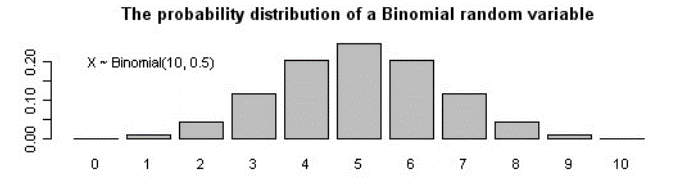
\includegraphics[width=1\linewidth]{binomial}}

\subsection{Negative Binomial Distribution, $NB(k, p)$ ($k^{th}$ success)}
\begin{itemize}
    \item Let X = no. of independent identical distributed Bernoulli(p) trials until \textbf{$k^{th}$ success} occurs.
    \item \textbf{Probability mass function of X}:
    \[P(X = x) = \binom{x-1}{k-1} p^k (1-p)^{x-k}\]
    \item \textbf{Notation}: $X \sim NB(k, p)$
    \item $E(X) = \frac{k}{p}$ and $V(X) = \frac{(1-p)k}{p^2}$
\end{itemize}

\subsection{Geometric Distribution, $G(p)$ (till $1^{st}$ success)}
\begin{itemize}
    \item Let X = no. of i.i.d. Bernoulli(p) trials until 1st success occurs.
    \[P(X = x) = p (1-p)^{x-1}\]
    \item \textbf{Notation}: $X \sim G(p)$
    \item $E(X) = \frac{1}{p}$ and $V(X) = \frac{1-p}{p^2}$
\end{itemize}

\columnbreak

\subsection{Poisson Distribution}
\begin{itemize}
    \item \textbf{Poisson RV}: Denotes number of events occuring in \textbf{fixed period of time or fixed region}, $k$ = no. of occurences.
    \[P(X = k) = \frac{e^{-\lambda}\lambda^k}{k!}\]
    \item \textbf{Notation}: $X \sim Poisson(\lambda)$ where $\lambda > 0$ is expected number of occurrences during given period/region
    \item $E(X) = \lambda$ and $V(X) = \lambda$
\end{itemize}
\centerline{\includegraphics[width=1\linewidth]{poisson}}
\centerline{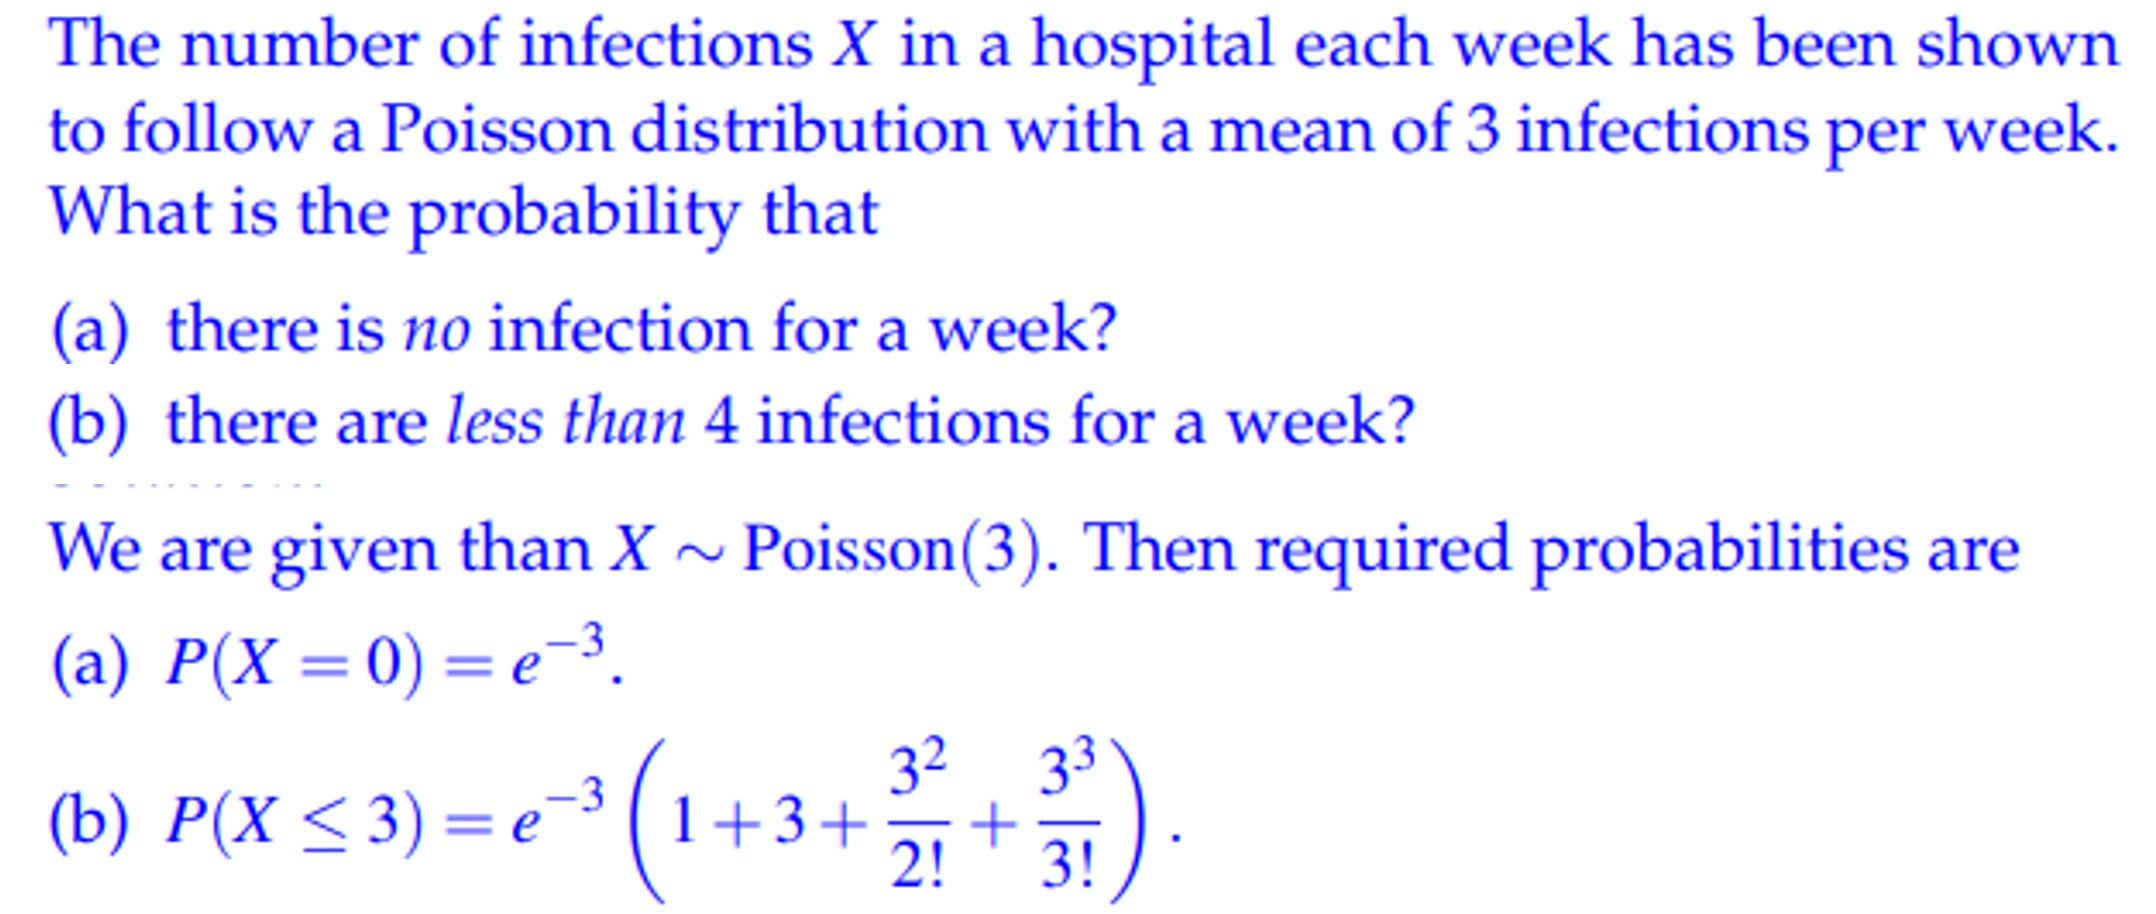
\includegraphics[width=0.8\linewidth]{poissonex}}
\subsubsection{Poisson Process}
\begin{itemize}
    \item Continuous time process, count number of occurrences within some interval of time. (given \textbf{rate} $\alpha$)
    \item Properties of \textbf{Poisson process with rate parameter} $\alpha$:
    \begin{itemize}
        \item Expected no. of occurrences in interval length $T$: $\alpha T$
        \item No simultaneous occurrences, and no. of occurrences in disjoint intervals independent.
    \end{itemize}
    \item \textbf{Number of occurrences in any interval} $T$ of Poisson process follows $Poisson(\alpha T)$ distribution. \\ (\textbf{Apply $X ~ Poisson(\alpha T)$ directly)}
\end{itemize}

\subsubsection{Poisson Approximation of Binomial Distribution}
\begin{itemize}
\item Let $X \sim B(n, p)$. Suppose $n \to \infty$ and $p \to 0$ s.t. $\lambda = np$ remains constant. \\
\item Then, approximately, $X \sim Poisson(\lambda)$.
\[\lim _{p \to 0; n \to \infty} P(X = x) = \frac{e^{-np} (np)^x}{x!}\]
\item Approximation is good when ($n \geq 20$ and $p \leq 0.05$), or ($n \geq 100$ and $np \leq 10$)
\end{itemize}



% CONTINUOUS==============
\section{4.2 Special Probability Distributions}
\begin{itemize}
\item \textbf{Continuous Distributions}: Many ``natural'' RVs whose set of possible values \textbf{uncountable}. Model with classes of continuous random variables.
\end{itemize}


\subsection{Continuous Uniform Distribution, $U(a,b)$}
RV X follows uniform distribution over interval $(a,b)$ if $p.d.f.$ given by:
\[f_X (x) = 
\begin{cases}
    \frac{1}{b-a} & a \leq x \leq b\\
    0 & otherwise
\end{cases}
\]
\begin{itemize}
    \item \textbf{Notation}: $X \sim U(a, b)$
    \item $E(X) = \frac{a+b}{2}$ and $V(X) = \frac{(b-a)^2}{12}$ \\ (derive by integration).
    \item \textbf{Cumulative distr. func.} $c.d.f.$ is given by:
    \[F_X (x) = 
    \begin{cases}
        0 & x < a\\
        \frac{x-a}{b-a} & a \leq x \leq b\\
        1 & x > b
    \end{cases}
    \]
\centerline{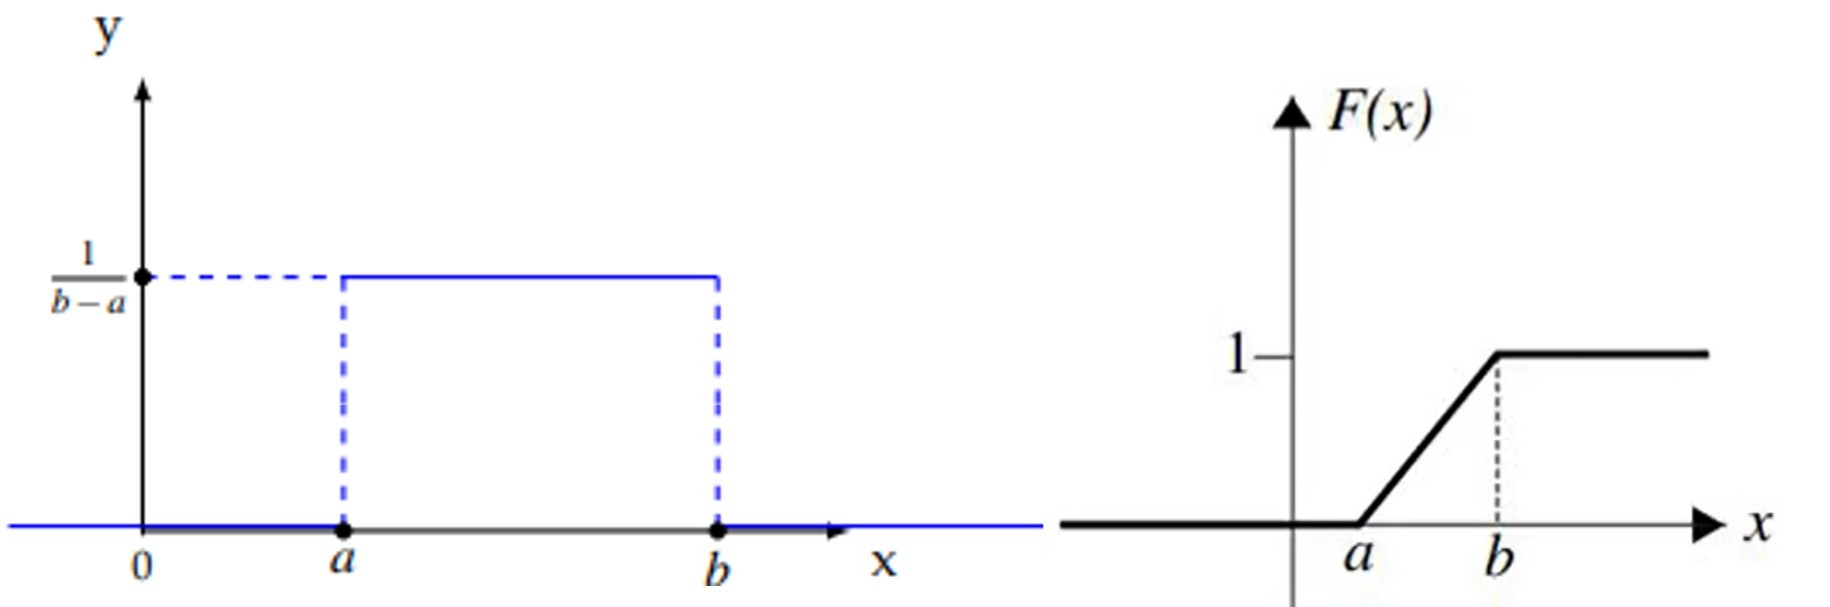
\includegraphics[width=1\linewidth]{uniformcd}}
\end{itemize}


\subsection{Exponential Distribution, $Exp(\lambda)$}
\begin{itemize}
\item Continuous counterpart to \textbf{geometric distribution}. 
\end{itemize}
X follows exponential distribution, with parameter $\lambda > 0$ if $p.f.$ is given by:
\[f_x (x) = 
\begin{cases}
    \lambda e^{-\lambda x} & x \geq 0\\
    0 & x < 0
\end{cases}\]
\begin{itemize}
    \item \textbf{Notation}: $X \sim Exp(\lambda)$
    \item $E(X) = \frac{1}{\lambda}$ and $V(X) = \frac{1}{\lambda^2}$
\centerline{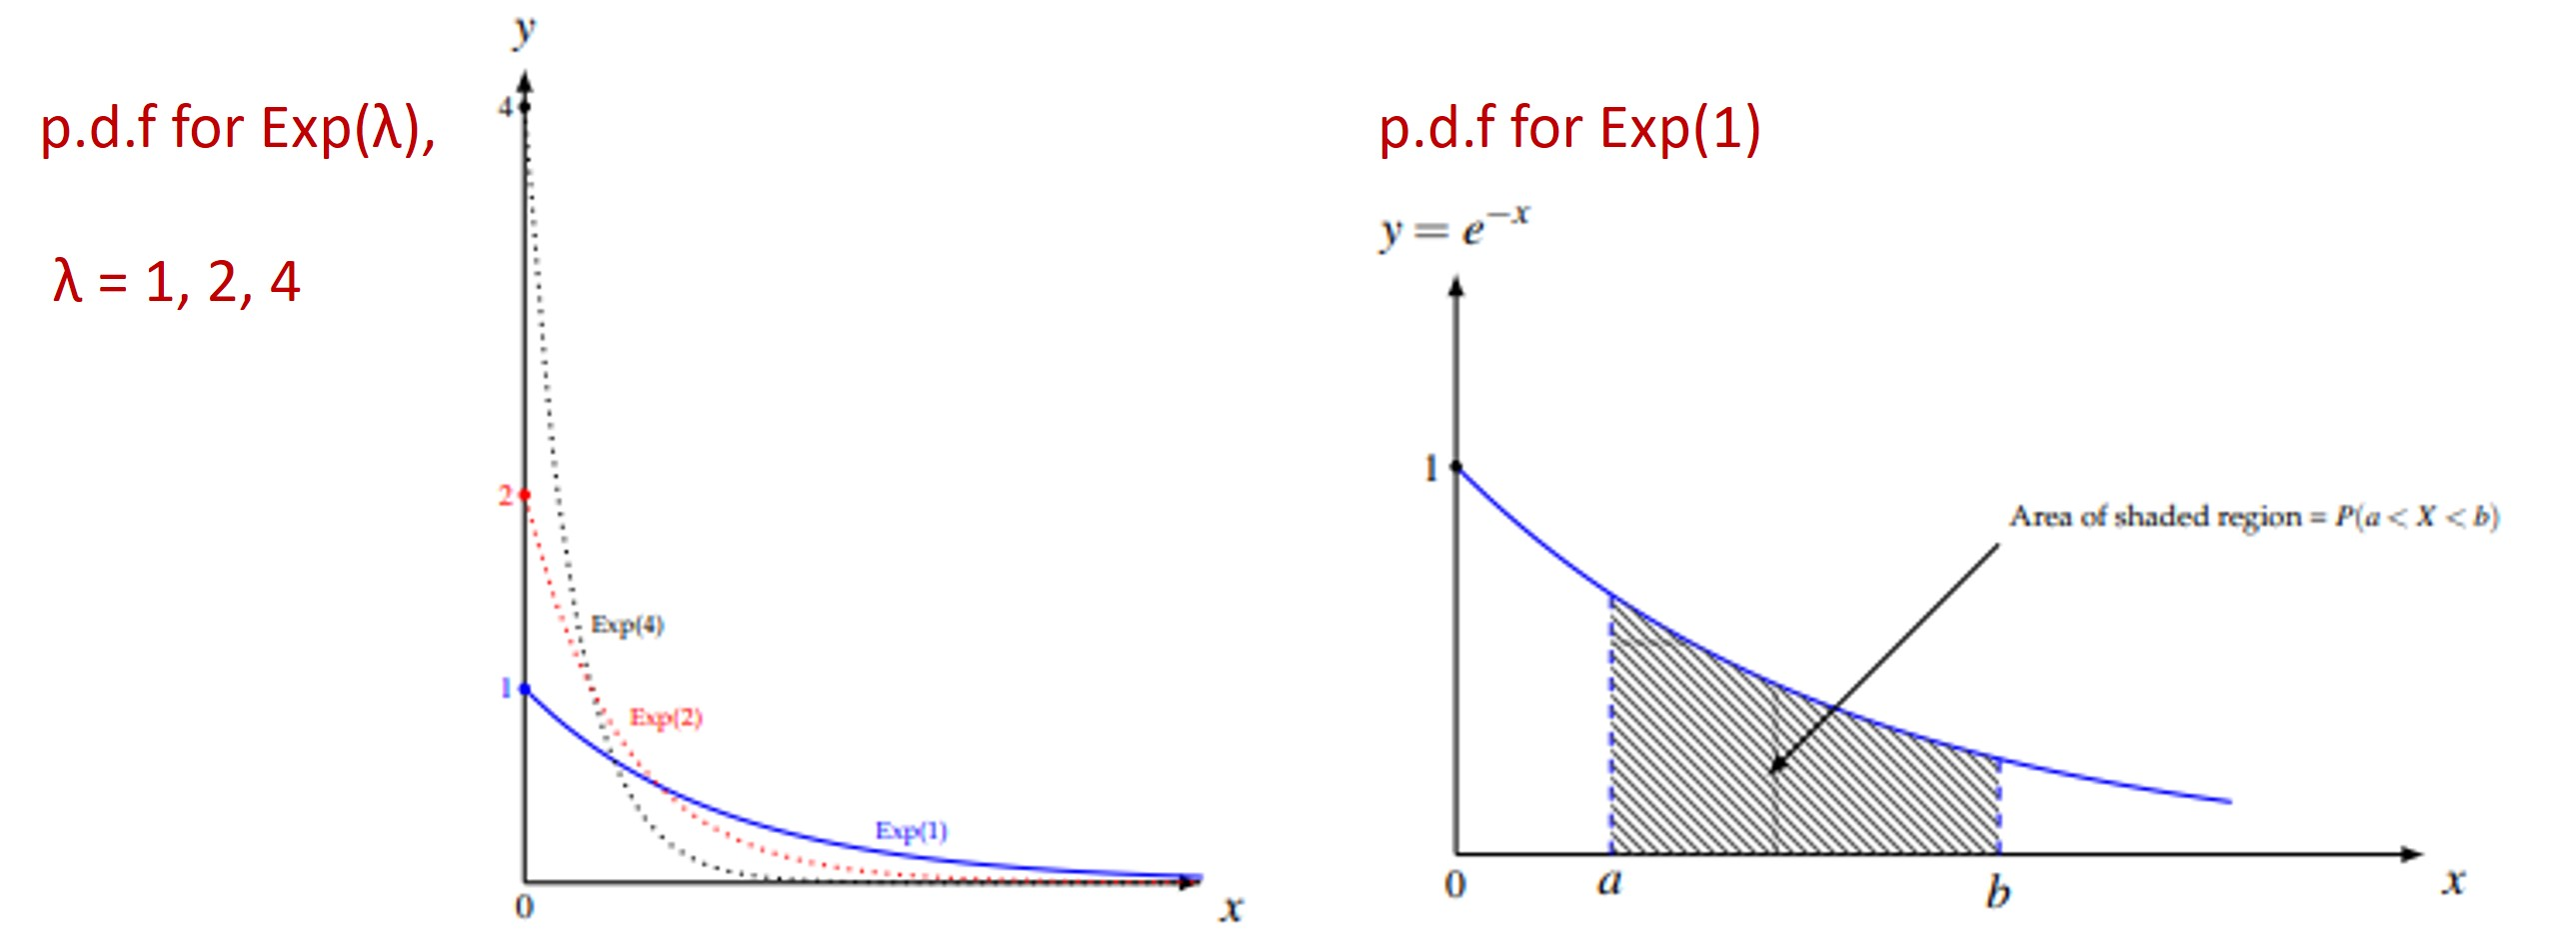
\includegraphics[width=0.8\linewidth]{exponential}}
	\item We can \textbf{derive $\lambda$ from mean / expectation of X}, since $E(X) = \frac{1}{\lambda}$.
    \item $c.d.f.$ is given by:
    \[F_X (x) = P(X \leq x) = 
    \begin{cases}
        1 - e^{-\lambda x} & x > 0\\
        0 & x \leq 0\\
    \end{cases}
    \]
    \item Additionally, $P(X > x) = e^{- \lambda x}$, for $x > 0$.
    \item \textbf{Exponential distribution ``Memoryless''}: Suppose $X$ has exponential distribution with $\lambda > 0$. Then for any positive numbers $s$ and $t$, we have:
    \[P(X > s+t | X > s) = P(X > t)\]
\end{itemize}

\subsection{Normal Distribution,  $N(\mu, \sigma^2)$}

X said to follow normal distribution with mean $\mu$ and variance $\sigma^2$ if $p.f.$ given by:
\[f_X (x) = \frac{1}{\sqrt{2 \pi} \sigma}e^{-(x-\mu)^2 / (2 \sigma ^2)}\]

\begin{itemize}
    \item \textbf{Notation}: $X \sim N(\mu, \sigma^2)$
    \item $E(X) = \mu$ and $V(X) = \sigma^2$
    \item $p.f.$ is \textbf{bell-shaped curve and symmetric} about $x = \mu$
    \item Total area under curve is 1
    \item 2 normal curves are identical in shape if they have same $\sigma ^2$. They differ in location by $\mu_1 - \mu_2$.
    \item As $\sigma$ increases, curve becomes more spread out
    \item If $X \sigma N(\mu, \sigma^2)$ and let $Z = \frac{X - \mu}{\sigma}$
\end{itemize}
\centerline{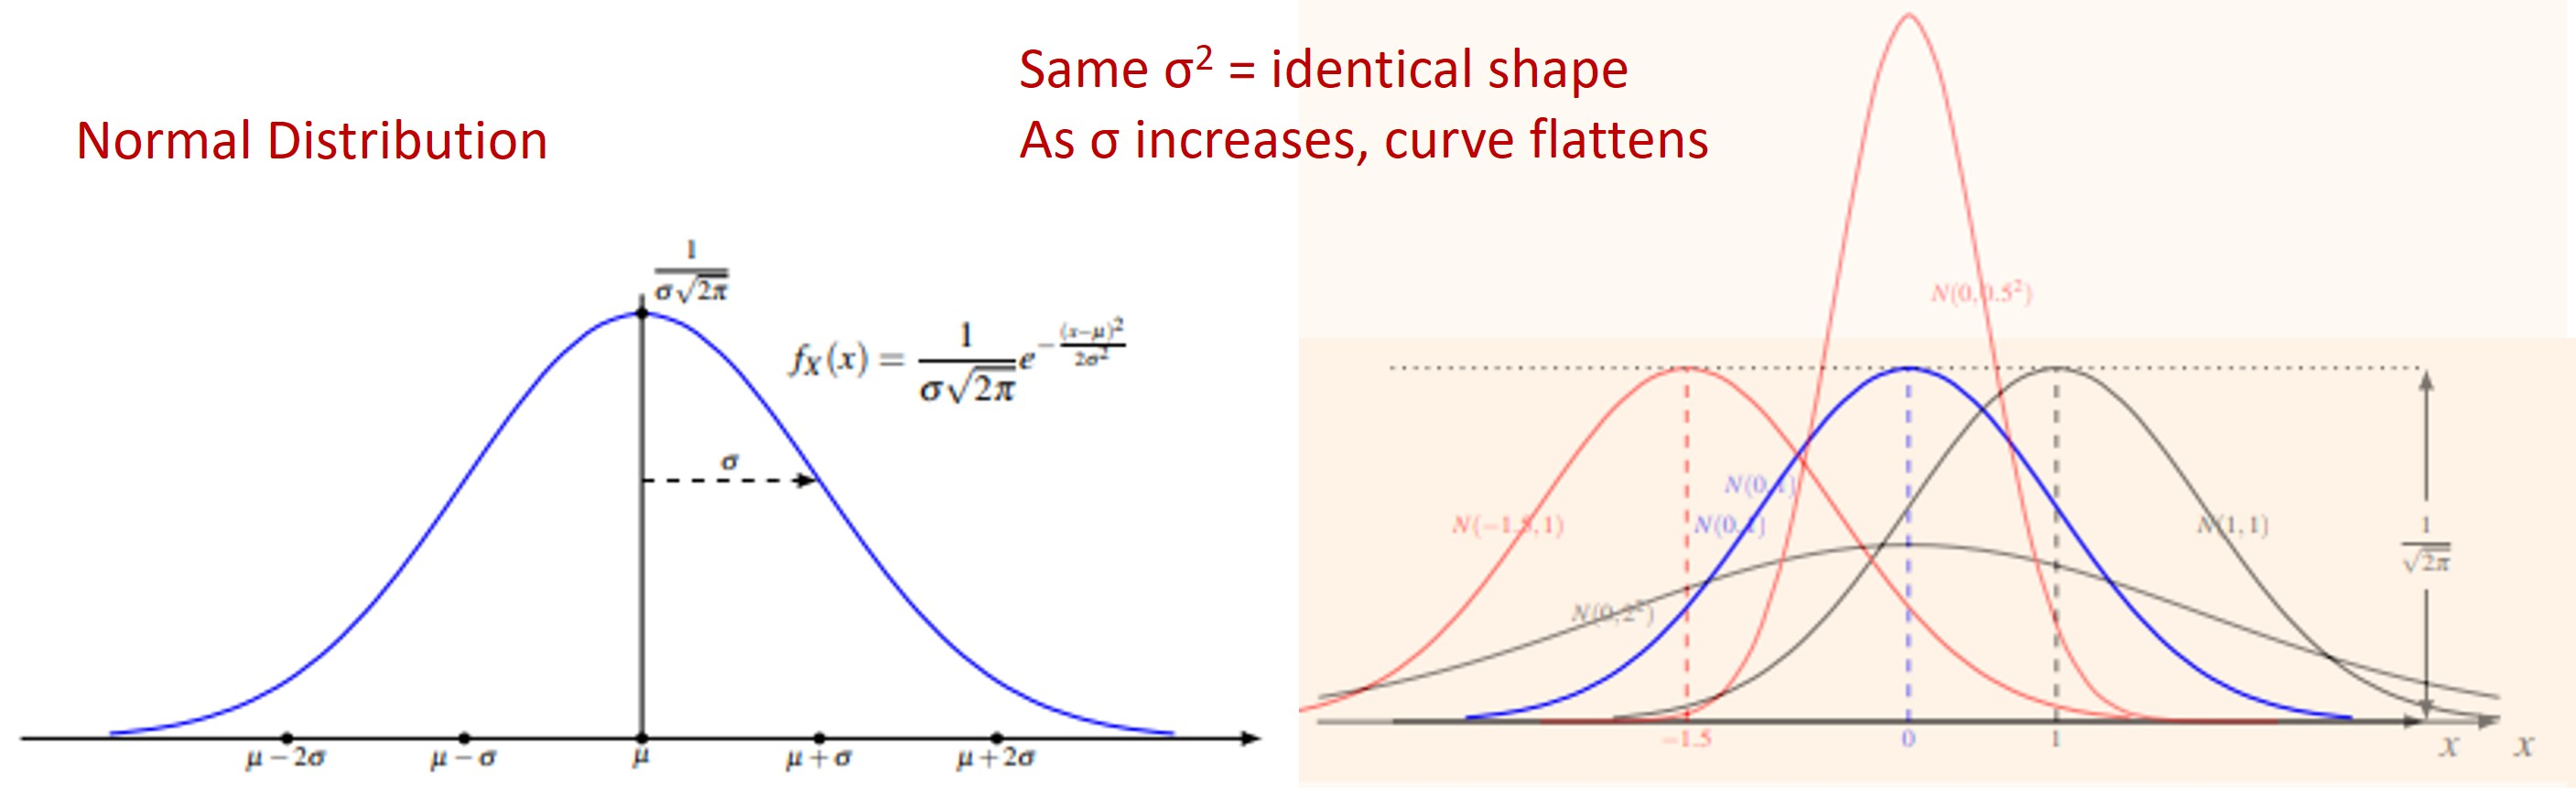
\includegraphics[width=1\linewidth]{normal}}

% \columnbreak


\subsubsection{Standardized Normal Distribution, $Z = N(0, 1)$}
If $X \sim N(\mu, \sigma ^2)$, then  $Z \sim N(0, 1)$:
\[Z = \frac{X - \mu}{\sigma}\]

\begin{itemize}
    \item $E(Z) = 0$ and $V(Z) = 1$
    \item \textbf{$p.f$ of $Z$ is given by}:
	\[\phi(z) = f_Z (z) = \frac{1}{\sqrt{2 \pi}} e^{-z^2 / 2}\]
\end{itemize}
\begin{itemize}
    \item \textbf{Standardizing normal distribution} allows us to use tables to find probabilities:
    \item For $X \sim N(\mu, \sigma^2)$, compute $P(x_1 < X < x_2)$ by standardization:
    \[x_1 < X < x_2 \leftrightarrow \frac{x_1 - \mu}{\sigma} < \frac{X - \mu}{\sigma} < \frac{x_2 - \mu}{\sigma}\]
    \item Then, $P(z_1 < Z < z_2)$, \textbf{use $f_Z (z)$ table to calculate}.   
 \end{itemize}
 
\begin{itemize}   
    \item \textbf{Cumulative d.f. of standard Normal}:
    \[\Phi(z) = F_Z (z) = \int _{-\infty} ^{z} f_Z (z) = \frac{1}{\sqrt{2 \pi}}\int _{-\infty} ^{z} e^{-t^2 / 2} dt\]
    \item $P(Z \geq 0) = P(Z \leq 0) = \phi(0) = 0.5$
    \item For any $z$, $\Phi(z) = P(Z \leq z) = P(Z \geq -z) = 1-\phi(-z)$
    \item $-Z \sim N(0, 1)$
    \item If $Z \sim N(0, 1)$, then $\sigma Z + \mu \sim N(\mu, \sigma^2)$
\end{itemize}
\subsubsection{Quantile}
\begin{itemize} 
    \item \textbf{Upper Quantile:} $x_\alpha$ that satisfies:
    \[P(X \geq x_\alpha) = \alpha\]
    \item where  $ 0 \leq \alpha \leq 1$. \\
\centerline{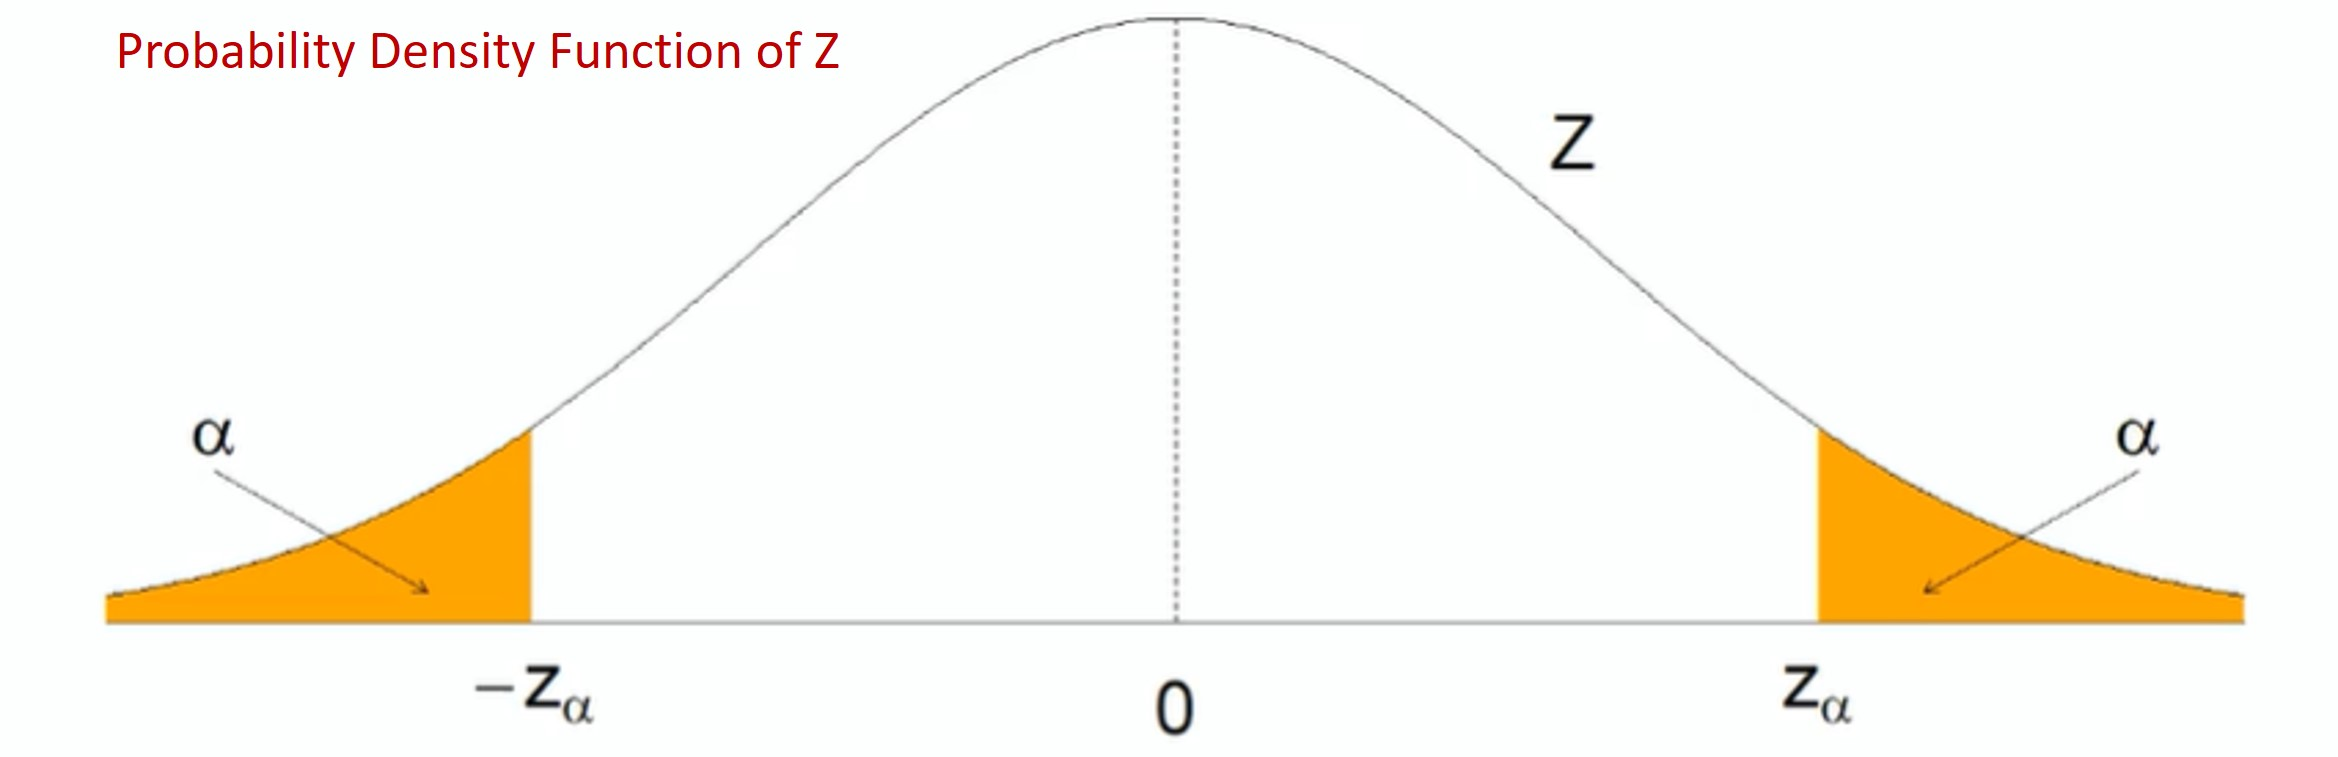
\includegraphics[width=0.6\linewidth]{upperquantile}}
    e.g. The 0.05th (upper) quantile of $Z \sim N(0,1)$ is 1.645, i.e. $z_{0.05} = 1.645$.
    \item $P(Z \geq z_\alpha) = P(Z \leq -z_\alpha) = \alpha$
    \item $\text{Upper } z_\alpha = \text{Lower } z_{1-\alpha}$
\end{itemize}

\subsubsection{Normal Approximation to Binomial Distribution}
Let $X \sim B(n, p)$, then as $n \to \infty$:
\[Z = \frac{X - E(X)}{\sqrt{V(X)}} = \frac{X - np}{\sqrt{np(1-p)}} \sim N(0, 1)\]

\begin{itemize}
    \item Approximation is good when $np > 5$ and $n(1-p) > 5$
\end{itemize}

\columnbreak

% Chapter 5==============
\section{5. Sampling, Sampling Distributions}


  
  
  
  
  
\end{multicols*}
\end{document}